\section{Features}
To specificy a more detailed design, the need for narrowing down the abstract states into features are required. The states are divided into feature groups, which can seen in \autoref{fig:design_diagram}. Each feature's functionality is defined by each outgoing action from the states the feature originates from. 
\begin{figure}[h]
	\centering
	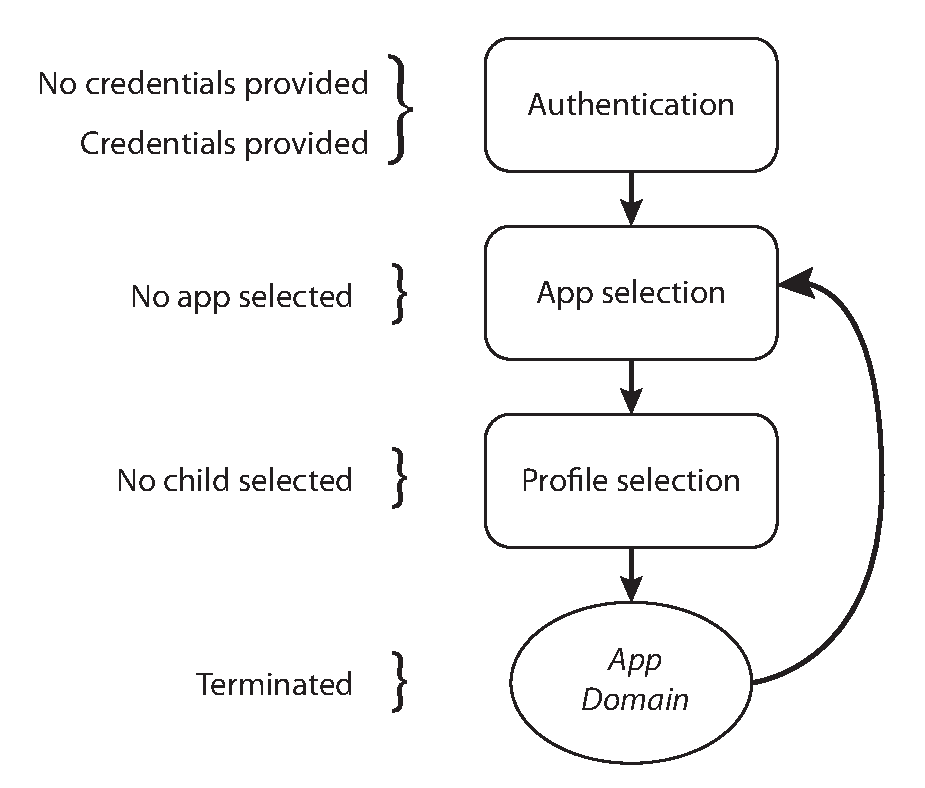
\includegraphics[width=1\textwidth]{gfx/design_diagram.pdf}
	\caption{Design diagram}
	\label{fig:design_diagram}
\end{figure}
\subsection{Authentication}
\begin{figure}[h]
	\centering
	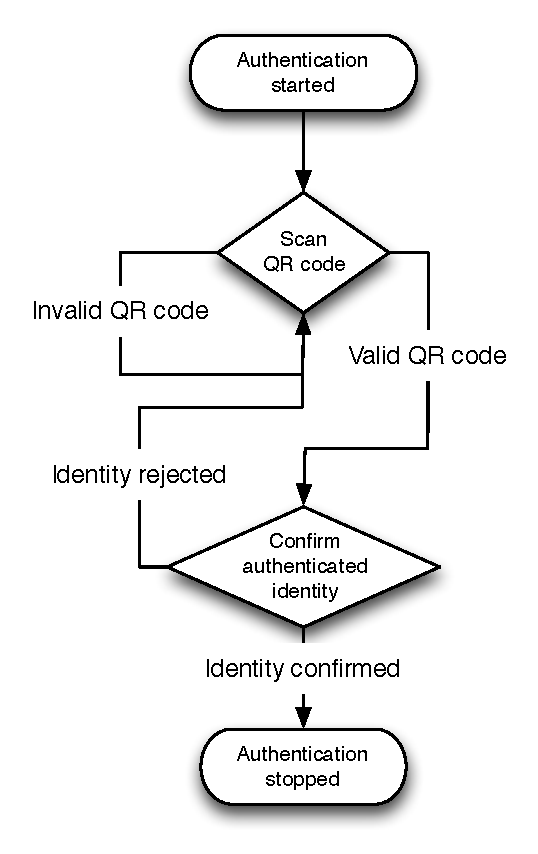
\includegraphics[width=0.5\textwidth]{gfx/authentication_design.pdf}
	\caption{Features of the Authentication functionality}
	\label{fig:authentication_design}
\end{figure}
\subsection{App selection}
\begin{figure}[h]
	\centering
	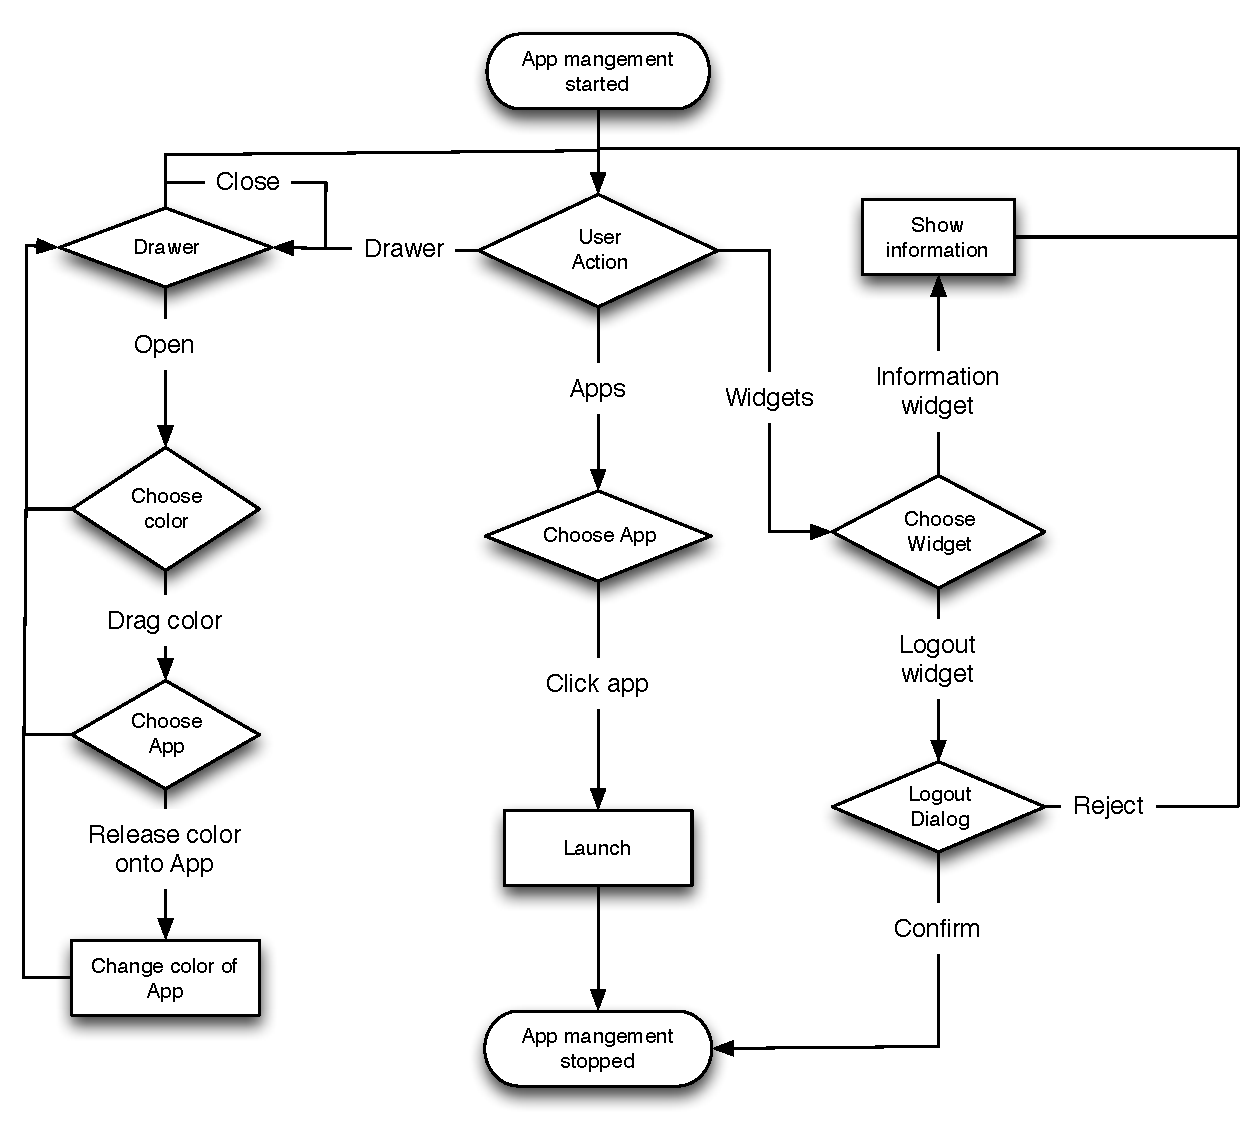
\includegraphics[width=0.7\textwidth]{gfx/appmanagement.pdf}
	\caption{Features of the App selection functionality}
	\label{fig:appselection_design}
\end{figure}
\subsection{Profile selection}
\begin{figure}[h]
	\centering
	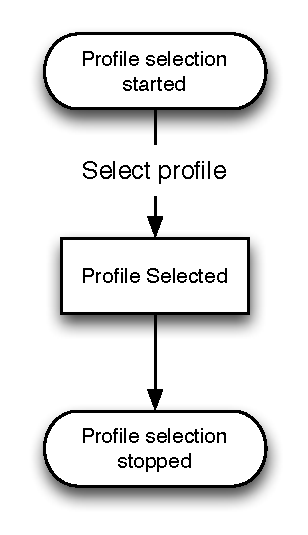
\includegraphics[width=0.3\textwidth]{gfx/profileselect_design.pdf}
	\caption{Features of the Profile selection functionality}
	\label{fig:profileselection_design}
\end{figure}